\documentclass[aspectratio=169]{beamer}
\usepackage{preamble_beamer}

\usetheme{Madrid}
\usefonttheme{professionalfonts}
\usepackage{amsmath, amssymb, amsthm}
\usepackage{tikz}
\usetikzlibrary{trees, positioning}
\usepackage{pgfplots}
\pgfplotsset{compat=1.18}
\usepackage{booktabs}

\newcommand*{\QEDB}{\null\nobreak\hfill\ensuremath{\square}}

\newtheorem*{question*}{Вопрос}
\newtheorem*{claim*}{Утверждение}

\title[Биноминальные и триноминальные деревья]{Лекция 8. Численные методы} % The short title appears at the bottom of every slide, the full title is only on the title page

\begin{document}

\begin{frame}
\titlepage
\end{frame}

% Секция 1: Биномиальные/триномиальные деревья
% \section{Биномиальные и триномиальные деревья}

\begin{frame}{Биномиальное дерево: конструкция}
\begin{block}{Параметры модели}
Для $S_t$ в модели Блэка-Шоулза:
\begin{itemize}
\item Вверх: $u = e^{\sigma\sqrt{\Delta t}}$
\item Вниз: $d = e^{-\sigma\sqrt{\Delta t}} = 1/u$
\item Вероятность: $p = \frac{e^{r\Delta t} - d}{u - d}$
\end{itemize}
\end{block}

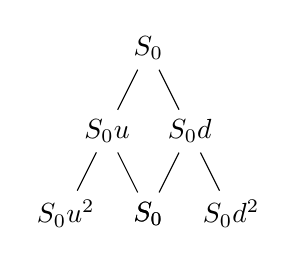
\begin{tikzpicture}[scale=0.7]
\node at (0,0) {$S_0$}
child {node {$S_0u$}
child {node {$S_0u^2$}}
child {node {$S_0$}}
}
child {node {$S_0d$}
child {node {$S_0$}}
child {node {$S_0d^2$}}
};
\end{tikzpicture}
\end{frame}

\begin{frame}{Биномиальное дерево: конструкция}
    \begin{itemize}
        \item Динамика
        $$
            S_{t+1} = \begin{cases} 
                S_t \cdot u, \text{ с вер. } q\\
                S_t \cdot d, \text{ с вер. } 1-q\\
            \end{cases}
        $$где $u=e^{r\tau + \sigma \sqrt{\tau}}$, $d=r^{r\tau - \sigma \sqrt{\tau}}$.
        \item Moment-matching:
        \begin{align*}
            &\E [S_{t + 1} | S_t] = e^{r\tau} S_t \to \\
            &u \cdot q + d \cdot (1 - q) = e^{r\tau} \to \\
            &q = \dfrac{e^{r\tau} - d}{u-d}
        \end{align*}
    \end{itemize}
\end{frame}

\begin{frame}{123}
     \begin{block}{Моделька}
        Динамика 
        $$
            S_{t+1} = \begin{cases} 
                S_t \cdot u, \text{ с вер. } q\\
                S_t \cdot d, \text{ с вер. } 1-q\\
            \end{cases}
        $$где 
        
        $$u=e^{r\tau + \sigma \sqrt{\tau}}$$
        $$d=r^{r\tau - \sigma \sqrt{\tau}}$$

        $$q = \dfrac{e^{r\tau} - d}{u-d}$$
    \end{block}
\end{frame}

\begin{frame}{Европейский опцион}
    \begin{itemize}
        \item Терминальное значение
        $$
            V_T = \Phi(S_T)
        $$
        \item Динамика
        \begin{align*}
            V_t(S_t) &= e^{-r\tau} \E^\Q [V_{t+1}(S_{t+1}) | S_t] = \\
            &= e^{-r\tau} \left(
                q V_{t+1}(S_t \cdot u) + (1 - q) V_{t+1}(S_t \cdot d)
            \right)
        \end{align*}
    \end{itemize}
\end{frame}

\begin{frame}{Американский опцион}
    \begin{itemize}
        \item Терминальное значение
        $$
            V_T = \Phi(S_T)^+
        $$
        \item Continuation value
        \begin{align*}
            C_t(S_t) &= e^{-r\tau} \E^\Q [V_{t+1}(S_{t+1}) | S_t] = \\
            &= e^{-r\tau} \left(
                q V_{t+1}(S_t \cdot u) + (1 - q) V_{t+1}(S_t \cdot d)
            \right)
        \end{align*}
        \item Принимаем решение об экспирации
        $$        
            V_t(S_t) = \max(C_t(S_t), \Phi(S_T))
        $$
    \end{itemize}
\end{frame}

\begin{frame}{Триноминальное дерево}
    \begin{itemize}
        \item Динамика
        $$
            S_{t+1} = S_t e^{r\tau} \begin{cases} 
                u, \text{ с вер. } q_1\\
                1, \text{ с вер. } q_2\\ 
                d, \text{ с вер. } q_3
            \end{cases}
        $$где $u=e^{\sigma \sqrt{3 \tau}}$, $d=r^{- \sigma \sqrt{3 \tau}}$.
        \item Moment-matching:
        \begin{align*}
            &q_1 + q_2 + q_3 = 1 \\
            &u q_1 + q_2 + d q_3 = 1 \\
            &u^2 q_1 + q_2 + d^2 q_3 = e^{\sigma^2 \tau}
        \end{align*}
        \item Решение:
        \begin{align*}
            &q_1 = \dfrac{e^{\sigma^2 \tau} - 1}{(u-1)(u-d)} \\
            &q_3 = \dfrac{e^{\sigma^2 \tau} - 1}{(1-d)(u-d)} \\
            &q_2 = 1 - q_1 - q_3
        \end{align*}
    \end{itemize}
\end{frame}

\begin{frame}{Европейский опцион}
    \begin{itemize}
        \item Терминальное значение
        $$
            V_T = \Phi(S_T)
        $$
        \item Динамика
        \begin{align*}
            V_t(S_t) &= e^{-r\tau} \E^\Q [V_{t+1}(S_{t+1}) | S_t] = \\
            &= e^{-r\tau} \left(
                q_1 V_{t+1}(S_t e^{r\tau} \cdot u) + 
                q_2 V_{t+1}(S_t e^{r\tau}) + 
                q_3 V_{t+1}(S_t e^{r\tau} \cdot d)
            \right)
        \end{align*}
    \end{itemize}
\end{frame}

\begin{frame}{Американский опцион}
        \begin{itemize}
        \item Терминальное значение
        $$
            V_T = \Phi(S_T)
        $$
        \item Continuation value
        \begin{align*}
            V_t(S_t) &= e^{-r\tau} \E^\Q [V_{t+1}(S_{t+1}) | S_t] = \\
            &= e^{-r\tau} \left(
                q_1 V_{t+1}(S_t e^{r\tau} \cdot u) + 
                q_2 V_{t+1}(S_t e^{r\tau}) + 
                q_3 V_{t+1}(S_t e^{r\tau} \cdot d)
            \right)
        \end{align*}
        \item Принимаем решение об экспирации
        $$        
            V_t(S_t) = \max(C_t(S_t), \Phi(S_T))
        $$
    \end{itemize}
\end{frame}


\begin{frame}{Сходимость биномиального метода}

\end{frame}

\begin{frame}{Численное уравнение УРЧП}
    \begin{itemize}
        \item Уравнение БШ
        $$\frac{\partial V}{\partial t} + \frac{1}{2}\sigma^2S^2\frac{\partial^2 V}{\partial S^2} + rS\frac{\partial V}{\partial S} - rV &= 0$$
        \item Замена $x = \log S$, $u(\tau, x) = V(T - \tau, e^x)$
        $$
            \frac{\partial u}{\partial \tau} &= \frac{\sigma^2}{2}\frac{\partial^2 u}{\partial x^2} + \left(r - \frac{\sigma^2}{2}\right)\frac{\partial u}{\partial x} - ru
        $$
        \item Сеточные функции $u_i^n = u(\tau_n, x_i)$. $h = \sigma \sqrt{\Delta t}$
        \begin{align*}
            \frac{u_i^{n+1} - u_i^n}{\Delta t} &= \frac{\sigma^2}{2}\frac{u_{i+1}^n - 2u_i^n + u_{i-1}^n}{h^2} \\
            &+ \left(r - \frac{\sigma^2}{2}\right)\frac{u_{i+1}^n - u_{i-1}^n}{2h} - ru_i^n
            \end{align*}
    \end{itemize}
\end{frame}

\begin{frame}
    \begin{itemize}
        \item Операторная запись
        $$
            \dfrac{du}{d\tau} = Au - ru
        $$
        $$
            (Au)_i = \frac{\sigma^2}{2}\frac{u_{i+1} - 2u_i + u_{i-1}}{h^2}
            &+ \left(r - \frac{\sigma^2}{2}\right)\frac{u_{i+1} - u_{i-1}}{2h}
            = \alpha_i u_{i - 1} + \beta_i u_i + \gamma_i u_{i+1}
        $$
        \item Точное решение:
        $$
            u^{n + 1} = \exp((A - \mathbb{I} r) \Delta t) u^n 
        $$
        \item Явная схема:
        $$
            u^{n + 1} = e^{-r \Delta t} (\mathbb{I} + \Delta t A)u^n
        $$
        \item Неявная схема:
        $$
            u^{n + 1} = e^{-r \Delta t} (\mathbb{I} - \Delta t A)^{-1}u^n
        $$
        \item Схема с полусуммой:
        $$
            u^{n + 1} = e^{-r \Delta t}  (\mathbb{I} - 0.5 \Delta t A)^{-1} 
            (\mathbb{I} + 0.5 \Delta t A)u^n
        $$
    \end{itemize}
\end{frame}

\begin{frame}{Явная схема}
    \begin{itemize}
        \item Операторная запись
        $$
            u^{n + 1} = e^{-r \Delta t} (\mathbb{I} + \Delta t A)u^n
        $$
        $$
            u^{n+1}_i = e^{-r \Delta t} \left(
                \tau \alpha_i u_{i-1}^n + (1 + \tau \beta_i) u_i^n + \gamma_i u_{i+1}^n
            \right)
        $$
    \end{itemize}
\end{frame}

\begin{frame}{Неявная схема}
    \begin{itemize}
        \item Операторная запись
        $$
            (\mathbb{I} - \Delta t A) u^{n + 1} = e^{-r \Delta t} u^n
        $$
        $$
            \left(
                -\tau \alpha_i u_{i-1}^{n+1} + (1 - \tau \beta_i) u_i^{n+1} - \gamma_i u_{i+1}^{n+1}
            \right) = e^{-r \Delta t} u^n_i
        $$
    \end{itemize}
\end{frame}

\begin{frame}
    Выразим $u_i^{n+1}$:
    \begin{align*}
    u_i^{n+1} &= u_i^n + \Delta t\left[\frac{\sigma^2}{2h^2}(u_{i+1}^n - 2u_i^n + u_{i-1}^n)\right. \\
    &\left.+ \frac{r - \frac{\sigma^2}{2}}{2h}(u_{i+1}^n - u_{i-1}^n) - ru_i^n\right]
    \end{align*}

    Сгруппируем коэффициенты:
    \begin{align*}
    u_i^{n+1} = &\left[\frac{\Delta t}{h}\left(\frac{\sigma^2}{2h} - \frac{r - \frac{\sigma^2}{2}}{2}\right)\right] u_{i-1}^n \\
    + &\left[1 - \Delta t\left(\frac{\sigma^2}{h^2} + r\right)\right] u_i^n \\
    + &\left[\frac{\Delta t}{h}\left(\frac{\sigma^2}{2h} + \frac{r - \frac{\sigma^2}{2}}{2}\right)\right] u_{i+1}^n
    \end{align*}

    Обозначим коэффициенты:
    \begin{align*}
    A &= \frac{\Delta t}{h}\left(\frac{\sigma^2}{2h} - \frac{r - \frac{\sigma^2}{2}}{2}\right) \\
    B &= 1 - \Delta t\left(\frac{\sigma^2}{h^2} + r\right) \\
    C &= \frac{\Delta t}{h}\left(\frac{\sigma^2}{2h} + \frac{r - \frac{\sigma^2}{2}}{2}\right)
    \end{align*}

    Тогда: $u_i^{n+1} = A u_{i-1}^n + B u_i^n + C u_{i+1}^n$
\end{frame}

% Секция 2: Американские опционы
% % \section{Американские опционы}

\begin{frame}{Граница экспирации}
\begin{block}{Динамическое программирование}
Цена американского опциона:
\begin{align*}
V_t &= \max\left\{ e^{-r\Delta t}\mathbb{E}[V_{t+\Delta t}|\mathcal{F}_t], \text{выплата}(S_t) \right\}
\end{align*}
\end{block}

\begin{figure}
\begin{tikzpicture}
\draw[->] (0,0) -- (4,0) node[right] {$S$};
\draw[->] (0,0) -- (0,3) node[above] {$V$};
\draw[blue, thick] (0.5,0.5) .. controls (2,1.5) and (3,2) .. (3.5,2.5);
\draw[red, dashed] (2,0) -- (2,1.8) node[above] {Граница экспирации};
\node at (1,1) {Регион продолжения};
\node at (3,1) {Регион экспирации};
\end{tikzpicture}
\end{figure}
\end{frame}

% Секция 3: Связь с УРЧП
% % \section{Связь с УРЧП}

\begin{frame}{Уравнение Блэка-Шоулза}
\begin{block}{УРЧП и преобразования}
\begin{align*}
\frac{\partial V}{\partial t} + \frac{1}{2}\sigma^2S^2\frac{\partial^2 V}{\partial S^2} + rS\frac{\partial V}{\partial S} - rV &= 0 \\
\text{Замена: } x &= \ln S, \quad \tau = T - t \\
\frac{\partial u}{\partial \tau} &= \frac{\sigma^2}{2}\frac{\partial^2 u}{\partial x^2} + \left(r - \frac{\sigma^2}{2}\right)\frac{\partial u}{\partial x} - ru
\end{align*}
\end{block}
\end{frame}

\begin{frame}{Явная схема и деревья}
\begin{block}{Дискретизация}
При $h = \sigma\sqrt{\Delta t}$ (шаг по пространству):
\begin{align*}
\frac{u_i^{n+1} - u_i^n}{\Delta t} &= \frac{\sigma^2}{2}\frac{u_{i+1}^n - 2u_i^n + u_{i-1}^n}{h^2} \\
&+ \left(r - \frac{\sigma^2}{2}\right)\frac{u_{i+1}^n - u_{i-1}^n}{2h} - ru_i^n
\end{align*}
\end{block}

\begin{block}{Связь с триномиальным деревом}
Коэффициенты совпадают с вероятностями:
\begin{align*}
p_u &= \frac{\Delta t}{2}\left(\frac{\sigma^2}{h^2} + \frac{r - \sigma^2/2}{h}\right) \\
p_d &= \frac{\Delta t}{2}\left(\frac{\sigma^2}{h^2} - \frac{r - \sigma^2/2}{h}\right)
\end{align*}
\end{block}
\end{frame}

% Секция 4: Устойчивость
% % \section{Устойчивость}

\begin{frame}{Условная устойчивость явной схемы}
\begin{block}{Критерий Куранта-Фридрихса-Леви}
Для устойчивости:
\begin{align*}
\Delta t \leq \frac{h^2}{\sigma^2 + |r - \sigma^2/2|h}
\end{align*}
\end{block}

\begin{figure}
\begin{tikzpicture}
\begin{axis}[
xlabel=$t$,
ylabel=Ошибка,
width=0.7\textwidth
]
\addplot[blue, domain=0:0.9] {0.1*exp(2*x)};
\addplot[red, domain=0.9:1] {0.1*exp(2*x)};
\node at (axis cs:0.5,1) {Устойчиво};
\node at (axis cs:1.1,3) {Неустойчиво};
\end{axis}
\end{tikzpicture}
\end{figure}
\end{frame}

% Секция 5: Неявная схема
% % \section{Неявные схемы}

\begin{frame}{Неявная схема}
\begin{block}{Дискретизация}
\begin{align*}
\frac{u_i^{n+1} - u_i^n}{\Delta t} &= \frac{\sigma^2}{2}\frac{u_{i+1}^{n+1} - 2u_i^{n+1} + u_{i-1}^{n+1}}{h^2} \\
&+ \left(r - \frac{\sigma^2}{2}\right)\frac{u_{i+1}^{n+1} - u_{i-1}^{n+1}}{2h} - ru_i^{n+1}
\end{align*}
\end{block}

\begin{block}{Метод прогонки (Томаса)}
Трехдиагональная система:
\begin{align*}
a_iu_{i-1}^{n+1} + b_iu_i^{n+1} + c_iu_{i+1}^{n+1} = u_i^n
\end{align*}
Сложность $O(N)$ вместо $O(N^3)$ для гауссова исключения
\end{block}
\end{frame}

\begin{frame}{Устойчивость неявной схемы}
\begin{block}{Анализ устойчивости}
Для тестового уравнения $u_t = \lambda u_{xx}$:
\begin{align*}
\text{Усиливающий множитель: } G &= \frac{1}{1 + 4\lambda\frac{\Delta t}{h^2}\sin^2(kh/2)} \\
|G| &\leq 1 \quad \text{для всех } \Delta t, h
\end{align*}
\end{block}

\begin{figure}
\begin{tikzpicture}
\draw[->] (0,0) -- (3,0) node[right] {Re};
\draw[->] (0,-1.5) -- (0,1.5) node[above] {Im};
\draw[red] (0,0) circle (1);
\draw[blue, thick] (-2,0) -- (-1,0);
\node at (-1.5,-0.5) {Собственные значения};
\end{tikzpicture}
\end{figure}
\end{frame}

% Секция 6: Схема Кранка-Николсон
% % \section{Схема Кранка-Николсон}

\begin{frame}{Схема с полусуммой}
\begin{block}{Дискретизация второго порядка}
\begin{align*}
\frac{u_i^{n+1} - u_i^n}{\Delta t} &= \frac{1}{2}L(u^{n+1}) + \frac{1}{2}L(u^n) \\
L(u) &= \frac{\sigma^2}{2}\delta_x^2 u + \left(r - \frac{\sigma^2}{2}\right)\delta_x u - ru
\end{align*}
\end{block}

\begin{block}{Свойства}
\begin{itemize}
\item Безусловно устойчива
\item Второй порядок точности $O(\Delta t^2 + h^2)$
\item Требует решения системы уравнений на каждом шаге
\end{itemize}
\end{block}
\end{frame}

% Секция 7: Аналогия с ОДУ
% \section{Аналогия с ОДУ}

\begin{frame}{Модельная задача: $y' = Ay$}
\begin{block}{Точное решение}
\begin{align*}
y(t+\tau) = e^{A\tau}y(t)
\end{align*}
\end{block}

\begin{block}{Численные схемы}
\begin{itemize}
\item Явная Эйлера: $y^{n+1} = (I + A\tau)y^n$
\item Неявная Эйлера: $y^{n+1} = (I - A\tau)^{-1}y^n$
\item Кранк-Николсон: $y^{n+1} = (I - A\tau/2)^{-1}(I + A\tau/2)y^n$
\end{itemize}
\end{block}
\end{frame}

\begin{frame}{Анализ устойчивости}
\begin{block}{Спектральный радиус}
Схема устойчива если $\rho(G) \leq 1 + O(\tau)$
\begin{align*}
\text{Явная: } &|\lambda_A\tau + 1| \leq 1 \\
\text{Неявная: } &\left|\frac{1}{1 - \lambda_A\tau}\right| \leq 1 \quad \text{для Re}(\lambda_A) \leq 0 \\
\text{Кранк-Николсон: } &\left|\frac{1 + \lambda_A\tau/2}{1 - \lambda_A\tau/2}\right| \leq 1
\end{align*}
\end{block}

\begin{figure}
\begin{tikzpicture}
\begin{axis}[
xlabel=Re($\lambda\tau$),
ylabel=Im($\lambda\tau$),
width=0.7\textwidth
]
\addplot[blue, domain=-2:0] {sqrt(1 - (x+1)^2)};
\addplot[blue, domain=-2:0] {-sqrt(1 - (x+1)^2)};
\addplot[red, domain=-5:5] {0};
\addplot[green, domain=-5:5] {0};
\end{axis}
\end{tikzpicture}
\caption{Области устойчивости: синяя - явная, красная - неявная, зеленая - Кранк-Николсон}
\end{figure}
\end{frame}

\begin{frame}{Заключение}
\begin{block}{Ключевые моменты}
\begin{itemize}
\item Деревья = явные схемы для УРЧП
\item Американские опционы = свободная граница
\item Устойчивость критична для явных схем
\item Неявные схемы устойчивы но требуют решения систем
\item Схемы второго порядка дают лучшую сходимость
\end{itemize}
\end{block}

\begin{block}{Практические рекомендации}
\begin{itemize}
\item Биномиальные деревья: простота реализации
\item Триномиальные деревья: лучшая сходимость
\item Неявные схемы: для задач с большими $\Delta t$
\item Кранк-Николсон: баланс точности и устойчивости
\end{itemize}
\end{block}
\end{frame}

\begin{frame}{Линейное ОДУ}
    \begin{itemize}
        \item Линейное уравнение:
        $$
            \dfrac{dy}{dt} = \lambda y(t),
        $$ $\lambda \gg -1$.
        \item Точное решение:
        $$
            y(t + \tau) = e^{\lambda \tau} y(t)
        $$
        \item Свойства: $y(t) > 0 \forall t$. 
        \item Сеточные функции $y_k = y(k \cdot \tau)$. Схема Эйлера:
        $$
            \dfrac{y_{k+1} - y_k}{\tau} = \lambda y_k \to y_{k+1} = (1 + \tau \lambda) y_k
        $$
        \item Условие положительности:
        $$
            1 + \tau \lambda > 0 \to \tau < -\dfrac{1}{\lambda}
        $$
        \item Условие устойчивости:
        $$
            |1 + \tau \lambda| < 1 \to \tau < -\dfrac{2}{\lambda}
        $$
    \end{itemize}
\end{frame}

\begin{frame}{Линейное ОДУ: схема Эйлера}
    График для устойчивой схемы.
    
    График для неустойчивой схемы.
\end{frame}

\begin{frame}{Линейное ОДУ: неявная схема}
    \begin{itemize}
        \item Неявная схема Эйлера:
        $$
            \dfrac{y_{k+1} - y_k}{\tau} = \lambda y_{k+1} \to
        $$
        $$
            y_{k+1} = (1 - \tau \lambda)^{-1} y_k
        $$
        \item Неявная схема генерирует положительное решение $\forall \tau \geq 0$:
        $$ 
            1 - \tau \lambda \geq 0 \quad \forall \tau \geq 0
        $$
        \item Неявная схема безусловно устойчива:
        $$
            |1 - \tau \lambda| \geq 1 \quad \forall \tau \geq 0
        $$
        \item График сходимости
    \end{itemize}
\end{frame}

\begin{frame}{Схема с полусуммой}
    \begin{itemize}
        \item Схема с полусуммой:
        $$
            \dfrac{y_{k+1} - y_k}{\tau} = \dfrac{\lambda }{2}\left(y_k + y_{k+1}\right) \to
        $$
        $$
            y_{k + 1} = \left(1 - {\tau \lambda}/{2}\right)^{-1} 
            \left(1 + {\tau \lambda}/{2}\right) y_k
        $$
        \item Условие положительности:
        $$
            \tau < -\dfrac{2}{\lambda}
        $$
        \item Безусловная устойчивость:
        $$
            \dfrac{|1+\tau \lambda / 2|}{ 1-  \tau \lambda /2} \leq 1 \quad \forall \tau \geq 0
        $$
        \item График
    \end{itemize}
\end{frame}

\begin{frame}{Порядок точности}
    \begin{itemize}
        \item Схема Эйлера:
        $$
            e^{\lambda \tau} - (1 + \lambda \tau) = \dfrac{\lambda^2 \tau^2}{2} + \ldots = O(\tau^2)
        $$
        \item Неявная схема Эйлера:
        $$
            e^{\lambda \tau} - (1 - \lambda \tau)^{-1}
            = 1 + \lambda \tau + \dfrac{\lambda^2 \tau^2}{2} - (1 + \lambda \tau + \lambda^2 \tau^2) 
            + \ldots 
            = -\dfrac{\lambda^2 \tau^2}{2} + \ldots = O(\tau^2)
        $$
        \item Схема с полусуммой:
        $$
            \dfrac{1+\tau \lambda / 2}{ 1-  \tau \lambda /2}
            = (1+\tau \lambda / 2)(1+\tau \lambda / 2 + \tau^2 \lambda^2 / 4 + \ldots)
            = 1 + \tau \lambda + \tau^2 \lambda^2 / 2 + O(\tau^3)
        $$
        $$
            e^{\lambda \tau} - \dfrac{1+\tau \lambda / 2}{ 1-  \tau \lambda /2} = O(\tau^3)
        $$
    \end{itemize}
\end{frame}

\begin{frame}{Сравнение схем}
    \begin{table}
    \centering
        %\begin{tabular}{p{2cm}|c|c|c|}
        \begin{tabular}{|l|c|c|c|}
            \hline
            & \textbf{Явная} & \textbf{Неявная} & \textbf{Полусумма} \\
            \hline
            \textbf{Формула} & 
            $(1 + \lambda\tau)y_k$ & 
            $(1 - \lambda\tau)^{-1}y_k$ & 
            $(1 - \lambda \tau / 2)^{-1}(1 - \lambda \tau / 2)y_k$ \\
            \hline
            \textbf{Положительность} &
            $\tau \leq \frac{1}{|\lambda|}$ &
            Всегда & $\tau \leq \frac{2}{|\lambda|}$ \\
            \hline
            \textbf{Устойчивость} &
            Условная & Безусловная & Безусловная \\
            & $\tau \leq \frac{2}{|\lambda|}$ & $\checkmark$ & $\checkmark$ \\
            \hline
            \textbf{Локальная точность} &
            $O(\tau^2)$ & $O(\tau^2)$ & $O(\tau^3)$ \\
            \hline
            \textbf{Глобальная точность} &
            $O(\tau)$ & $O(\tau)$ & $O(\tau^2)$ \\
            \hline
        \end{tabular}
    \end{table}
\end{frame}

\begin{frame}{Системы линейных ОДУ}
    \begin{itemize}
    \item Линейное уравнение:
    $$
        \dfrac{dy}{dt} = A y(t),
    $$ $\lambda(A) < 0$.
    \item Точное решение:
    $$
        y(t + \tau) = e^{A \tau} y(t)
    $$
    где матричная экспонента задаётя как
    $$
        e^{A \tau} = \mathbb{I} + A\tau + \dfrac{(A\tau)^2}{2} + \ldots 
        = \sum_{n=0}^{\infty} \dfrac{(A\tau)^n}{n!}
    $$
    % \item Схема Эйлера:
    % $$
    %     y_{k+1} = (\mathbb{I} + \tau A) y_k
    % $$
    % \item Неявная схема:
    % $$
    %     y_{k+1} = (\mathbb{I} - \tau A)^{-1} y_k
    % $$
    % \item Схема с полусуммой:
    % $$
    %     y_{k+1} = (\mathbb{I} - \tau A / 2)^{-1} (\mathbb{I} + \tau A / 2) y_k
    % $$
    \end{itemize}
\end{frame}

\begin{frame}{Сравнение схем}
    \begin{table}
    \centering
        %\begin{tabular}{p{2cm}|c|c|c|}
        \begin{tabular}{|l|c|c|c|}
            \hline
            & \textbf{Явная} & \textbf{Неявная} & \textbf{Полусумма} \\
            \hline
            \textbf{Формула} & 
            $(\mathbb{I} + \tau A)y_k$ & 
            $(\mathbb{I} - \tau A)^{-1}y_k$ & 
            $(\mathbb{I} - \tau A / 2)^{-1}(\mathbb{I} + \tau A / 2)y_k$ \\
            \hline
            \textbf{Устойчивость} &
            Условная & Безусловная & Безусловная \\
            & $\tau \leq \frac{2}{|\max\lambda(A)|}$ & $\checkmark$ & $\checkmark$ \\
            \hline
            \textbf{Локальная точность} &
            $O(\tau^2)$ & $O(\tau^2)$ & $O(\tau^3)$ \\
            \hline
            \textbf{Глобальная точность} &
            $O(\tau)$ & $O(\tau)$ & $O(\tau^2)$ \\
            \hline
        \end{tabular}
    \end{table}
\end{frame}

\begin{frame}{Метод прогонки}
    \begin{itemize}
        \item Система с трёх-диагональной матрицей
        \begin{align*}
            & B_1 x_1 + C_1 x_2 = F_1\\
            & A_i x_{i-1} + B_i x_i + C_i x_{i + 1} = F_i, i = 2 \ldots N-1 \\
            & A_{N} x_{N-1} + B_N x_N = F_N
        \end{align*}
        \item Прямой проход:
        \begin{align*}
            &\alpha_1 = \beta_1 = 0\\
            &\alpha_{i+1} = \dfrac{-C_i}{A_i \alpha_i + B_i}, \quad 
            \beta_{i+1} = \dfrac{F_i - A_i \alpha_i}{A_i \alpha_i + B_i}
        \end{align*}
        \item Обратный проход:
        \begin{align*}
            &x_N = \dfrac{F_N - A_N \beta_N}{B_N + A_N + \alpha_N} \\
            &x_i = \alpha_{i + 1} x_i + \beta_{i + 1}, i=N-1 \ldots 1
        \end{align*}
    \end{itemize}
\end{frame}

\begin{frame}{Численные методы интегрирования}
    \begin{itemize}
        \item Задача: вычислить интеграл $I = \int_a^b f(x) dx$
        \item Схема правых прямоугольников:
        $$
            f(x) \approx f(a) \to I \approx f(a) \cdot (b - a)
        $$
        \item Схема левых прямоугольников:
        $$
            f(x) \approx f(b) \to I \approx f(b) \cdot (b - a)
        $$
        \item Схема средних:
        $$
            f(x) \approx f(c) \to I \approx f(c) \cdot (b-a)
        $$ где $c = \frac{a+b}{2}$ -- середина отрезка.
        \item Схема трапеций:
        $$
            f(x) \approx f(a) + (f(b) - f(a)) \cdot \dfrac{(x-a)}{b-a}
            \to I \approx 0.5 (f(a) + f(b)) \cdot (b-a)
        $$
    \end{itemize}
\end{frame}



\begin{frame}{Численное интегрирование}
    \begin{itemize}
        \item Хотим оценить интеграл:
        $$
            I = \int_a^b f(x) dx
        $$
        \item Замена переменных $x = a + (b - a) \cdot u$
        $$
            I  = \int_a^b f(x) dx = (b-a) \cdot \int_0^1 f(a + (b-a)\cdot u) du = 
            (b-a)\cdot \int_0^1 g(u) du
        $$
        \item Без ограничения общности считаем $a = 0, b = 1$.
        \item Апроксимация функции: 
        $$
            g(u) \approx \hat{g}(u), \;\; u \in [0, 1]
        $$
        \item Оценка интеграла:
        $$
            \hat{I} = \int_0^1 \hat{g}(u) du
        $$ 
    \end{itemize}
\end{frame}

\begin{frame}{Численное интегрирование: примеры}
    \begin{itemize}
        \item Схема правых прямоугольников:
        $$
            \hat{g}(u) = g(0) \to \hat{I} = g(0)
        $$
        \item Схема левых прямоугольников:
        $$
            \hat{g}(u) = g(1) \to \hat{I} = g(1)
        $$
        \item Схема средних:
        $$
            \hat{g}(u) = g(0.5) \to \hat{I} = g(0.5)
        $$
        \item Схема трапеций:
        $$
            \hat{g}(u) = g(0) + (g(1) - g(0)) \cdot u
            \to \hat{I} =0.5 (g(a) + g(b))
        $$
    \end{itemize}
\end{frame}

\begin{frame}{Квадратичная аппроксимация}
       \begin{itemize}
        \item Рассмотрим функцию $g(u), u \in [0, 1]$
        \item Квадратичная аппроксимация $\hat{g}(u)$:
        \begin{itemize}
            \item $\hat{g}(u)$ -- квадратичная функция
            \item $\hat{g}(u_j) = g(u_j)$, при $u_j \in \{0, 0.5, 1\}$ 
        \end{itemize}

        \item Базисные функции 
        \begin{align*}
            &h_1(u) = 2 (u - 1)(u - 0.5) \\
            &h_2(u) = 4 u (u - 1) \\
            &h_3(u) = 2 u (u - 0.5) 
        \end{align*}
        \item Свойства:
        $$
            h_i(u_j) = \delta_{ij} = \begin{cases}1, i = j \\ 0, i \neq j\end{cases}
        $$

        \item Квадратичная аппроксимация:
        $$
            \hat{g}(u) = g(0) h_1(u) + g(1) h_2(u) + g(0.5) h_3(u)
        $$
    \end{itemize} 
\end{frame}

\begin{frame}{Схема Симпсона}
    \begin{itemize}
        \item Квадратичная аппроксимация:
        $$
            \hat{g}(u) = g(0) h_1(u) + g(0.5) h_2(u) + g(1) h_3(u)
        $$
        \item Схема Симпсона:
        $$
            \hat{I} = \int_0^1 \hat{g}(u) du
            = g(0) I_1 + g(0.5) I_2 + g(1) I_3
        $$где $I_1 = I_2 = \dfrac{1}{6}, \; I_2 = \dfrac{4}{6}$
        $$
            \hat{I} = \dfrac{1}{6} \left( u(0) + 4 u(0.5) + u(1) \right)
        $$
    \end{itemize}
\end{frame}

\begin{frame}{Составные формулы Котеса}
    \begin{itemize}
        \only<1>{
        \item Пусть $N \in \mathbb{N}$. Разобъём отрезок $[0, 1]$ на малые отрезки длинной $h=\dfrac{1}{N}$
        \item Узлы сетки $u_i = i \cdot h, i=0,\ldots, N$
        \item Линейность интеграла по интервалу интегрирования:
        $$
            I = \int_0^1 g(u)du = \sum_{i=0}^{N-1} \int_{u_i}^{u_{i+1}} g(u) du
        $$
        \item На каждом интервале $[u_i, u_{i+1})$ воспользуемся одной из квадратурных формул $I_i \approx \hat{I}_i$
        \item Состовная формула для $\hat{I}$:
        $$
            \hat{I} = \sum_{i=0}^{N-1} \hat{I}_i
        $$}
        \only<2->{\item Составная формула левых/правых/средних прямоугольников:
        $$  
            \hat{I} = \sum_{i=0}^{N-1} g(c_i) \cdot h
        $$
        где 
            $$
            c_i = \begin{cases}
                u_i, \text{ для левых прямоугольников} \\
                u_{i+1}, \text{ для правых прямоугольников} \\
                u_i + h/2, \text{ для средних}
            \end{cases}
        $$
            \item Состовная формула трапеций
            $$
                \hat{I} = h\cdot \left(
                    0.5 g(u_0) + \sum_{i=1}^{N-1} g(u_i) + 0.5 g(u_N)
                \right)
            $$
        }
    \end{itemize}
\end{frame}

\begin{frame}{Погрешность метода средних}
    \begin{itemize}
        \only<1>{
        \item Рассмотрим составной метод средних:
        $$
            \hat{I} = \sum_{i=0}^{N-1} g(u_i + 0.5 h) \cdot h
        $$
        \item Ошибка на $i$-ом интервале:
        $$
            E_i = |I_i - \hat{I}_i|
            = \Bigm\vert\int_{u_i}^{u_{i+1}} (g(u) - g(c_i)) du\Bigm\vert
        $$ где $c_i = u_i + 0.5 h$}
        \only<1-2>{\item Разложим $g(u)$ в ряд тейлора в окрестности $c_i$:
        $$
            g(u) - g(c_i) = g^{\prime}(c_i) (u - c_i) + \dfrac{1}{2} g^{\prime\prime}(\xi) (u-c_i)^2
        $$ где $\xi \in [u_i, u_{i+1}]$}
        \only<2->{
        \item Рассмотрим интеграл по интервалу $[u_i, u_{i+1})$
        \begin{align*}
            &E_i = \Bigm\vert\int_{u_i}^{u_{i+1}} \left[ g^{\prime}(c_i) (u - c_i) + 
            \dfrac{1}{2} g^{\prime\prime}(\xi) (u-c_i)^2\right]du\Bigm\vert
            \leq \dfrac{1}{2} M_i\int_{u_i}^{u_{i+1}}(u-c_i)^2du = \dfrac{1}{24} M_i h^3
        \end{align*}где 
        $$
            M_i = \max_{u\in [u_i, u_{i+1}]} |g^{\prime\prime}(u)| 
        $$}
        \only<3>{
        \item Суммарная погрешность:
        $$
            E_N = \sum_{i=0}^{N-1} E_i = \dfrac{h^3}{24} \sum_{i=0}^{N-1} M_i
            \leq \dfrac{h^2}{24} M
        $$где $M = \max_i M_i = \max_{u\in[0, 1]} ||g^{\prime\prime}(u)||$}
    \end{itemize}
\end{frame}

\begin{frame}{Сравнение квадратурных формул}
    \small
    \begin{table}
    \centering
    \begin{tabular}{|l|c|c|}
    \hline
    \textbf{Метод} & \textbf{Формула} & \textbf{Главный член ошибки} \\
    \hline
    Левые прямоугольники & 
    $h \sum\limits_{i=0}^{N-1} g(u_i)$ &
    $\dfrac{1}{2}h \cdot g'(\xi)$ \\
    \hline
    Правые прямоугольники & 
    $h \sum\limits_{i=0}^{N-1} g(u_{i+1})$ &
    $-\dfrac{1}{2}h \cdot g'(\xi)$ \\
    \hline
    Средние прямоугольники & 
    $h \sum\limits_{i=0}^{N-1} g(u_i + \frac{h}{2})$ &
    $\dfrac{1}{24}h^2 \cdot g''(\xi)$ \\
    \hline
    Формула трапеций & 
    $h \sum\limits_{i=0}^{N-1} \dfrac{g(u_i) + g(u_{i+1})}{2}$ &
    $-\dfrac{1}{12}h^2 \cdot g''(\xi)$ \\
    \hline
    Формула Симпсона & 
    $\dfrac{h}{3} \left[g(u_0) + g(u_N) + 4\sum\limits_{\text{неч.}} g(u_i) + 2\sum\limits_{\text{чет.}} g(u_i)\right]$ &
    $-\dfrac{1}{180}h^4 \cdot g^{(4)}(\xi)$ \\
    \hline
    \end{tabular}
\end{table}
\end{frame}


\begin{frame}{Апостериорная оценка погрешности}
    \begin{itemize}
        \item Хотим оценить ошибку, не зная точного решения
        \item Ошибка имеет степенную зависимость от шага сетки $h = \dfrac{1}{N}$
        $$
            I_N = I + R_N = I + c \cdot h^{p}
        $$где $R_N$ -- ошибка на $N$ узлах, $c\in \R$ -- константа, $p$ -- порядок метода.
        \item Оценка на сгущённой сетке:
        $$
            I_{2N} = I + R_{2N} = I + \dfrac{c}{2^p} \cdot h^p
        $$
        \item Вычтем второе уравнение из первого, получим:
        $$
            I_{2N} - I_N = \dfrac{c}{2^p} \cdot h^p - c \cdot h^{p} = R_{2N}(1 - 2^p)
        $$откуда оценка ошибки: 
        $$
            R_{2N} = \dfrac{I_N - I_{2N}}{2^p - 1}
        $$
    \end{itemize}
\end{frame}

\begin{frame}{Улучшение точности}
    \begin{itemize}
    \item Зная оценку ошибки $\hat{R}_N$ можем получить более точную оценку для интеграла:
    $$
        \hat{I}_N = I_N - \hat{R}_N 
    $$
    \item Ошибка $\hat{I}_N$ имеет более высокий порядок чем $p$. Для несимметричных схем:
    $$
        \hat{I}_N = I_N - \hat{R}_N = I + c' h^{p+1}
    $$
    \item Для симметричных схем ошибка расскладывается по чётным степеням $h$:
    $$
        \hat{I}_N = I_N - \hat{R}_N = I + c'' h^{p+2}
    $$
    \item Улучшение точности можно проделывать много раз
    \end{itemize}
\end{frame}

\end{document}
